% begin module fermats-theorem-does-not-say
\begin{frame}[t]
\begin{theorem}[Fermat's Theorem]
If $f$ has a local maximum or minimum at $c$, and if $f'(c)$ exists, then $f'(c) = 0$.
\end{theorem}
What does Fermat's Theorem not say?
\uncover<2->{%
\begin{example}[Example 3, p. 263]
\begin{columns}[c]
\column{.4\textwidth}
\ 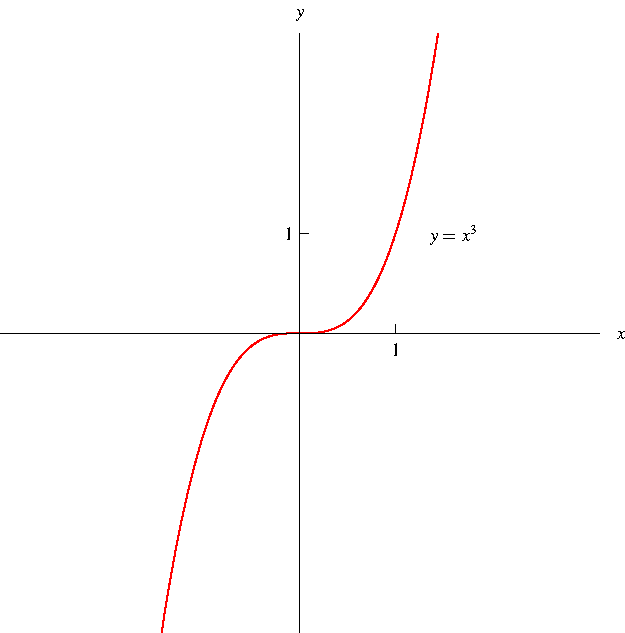
\includegraphics[width=3cm]{maxima-minima/pictures/01-02-xcubed.pdf}%
\column{.6\textwidth}
\begin{itemize}
\item<2->  Let $f(x) = x^3$.
\item<3-| alert@4-5>  Then $f'(x) = \uncover<5->{3x^2.}$
\item<3-| alert@6-7>  $f'(x) = 0$ when $x = \uncover<7->{0.}$
\item<8->  But $f$ has no local maximum or minimum at 0!
\end{itemize}
\end{columns}
\end{example}
}%

\uncover<9->{Fermat's Theorem does not say ``if $f'(c) = 0$, then $f$ has a local maximum or a local minimum at $c$.''}
\end{frame}



\begin{frame}[t]
\begin{theorem}[Fermat's Theorem]
If $f$ has a local maximum or minimum at $c$, and if $f'(c)$ exists, then $f'(c) = 0$.
\end{theorem}
What does Fermat's Theorem not say?
\uncover<2->{%
\begin{example}[Figure 12, p. 265]
\begin{columns}[c]
\column{.45\textwidth}
\ 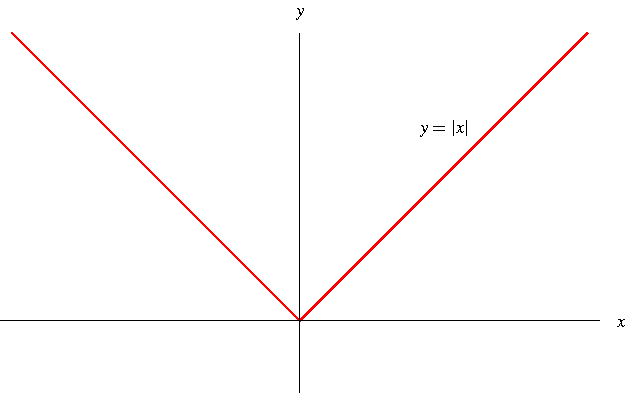
\includegraphics[width=6cm]{maxima-minima/pictures/04-01-abs.pdf}%
\column{.55\textwidth}
\begin{itemize}
\item<2->  Let $f(x) = |x|$.
\item<3-| alert@3-4>  Then $f$ has a local minimum at \uncover<4->{$0$.}
\item<5->  But $f'(0)$ doesn't exist!
\end{itemize}
\end{columns}
\end{example}
}%

\uncover<6->{Fermat's Theorem does not say ``if $f$ has a local maximum or minimum at $c$, then $f'(c)$ exists.''}
\end{frame}
% end module fermats-theorem-does-not-say
